\section{Introduction}
In this chapter, in section \ref{sec:nosql}, NoSQL databases are firstly introduced and compared with SQL solutions. In section \ref{sec:common-language} are listed some of the solution that has been developed in defining a common language or interface to interact with different NoSQL databases.

\noindent In section \ref{sec:jpa} is described the JPA interface and JPQL the query language used for JPA queries. In section \ref{sec:cpim} the CPIM library is introduced as a tentative in defining a common interface to interacts with different vendors in a PaaS environment, which include accessing their NoSQL solution.

\section{NoSQL databases}
\label{sec:nosql}
\subsection{NoSQL motivations}
\subsection{NoSQL characteristics}
\subsection{Standard language}
ORM (Object Relational Mapping) solutions came into existence to solve OO-impedance mismatching problem. Most popular among them are Hibernate, Toplink, EclipseLink etc. They worked beautifully with relational databases like Oracle and MySQL, among others.

Each ORM solution had its own API and object query language (like HQL for hibernate) which made it difficult for programmers to switch from one framework to another. As a result, efforts were made to make standards and specifications. 

Problem with NoSQL databases is that there is NOT EVEN ONE existing industry standard (like SQL) for them. The very basic idea of “something opposed to SQL”…and as a result – deviation from standards and rules, is going to be suicidal, if not corrected at right time. Learning to work with a new NoSQL database is always cumbersome as a result.

Apart from that, people lack in-depth knowledge of NoSQL. Even if they do, they are confined to one or two. In relational world, people depend upon their knowledge of SQL and JDBC to work on basic and intermediate database things. Switching to another database requires little or almost no effort, which otherwise is painful in NoSQL  world.

ORM for NoSQL is a bit mis-leading term. People prefer to call it “OM tool for NoSQL” or maybe “ODM – Object data-store Mapping tool”. ORM frameworks have already been there for 30+ years and it’s a de-facto industry standard. People are very clear about what ORM tools are supposed to do. There are no surprises.

Key here is to let people forget worrying about complexities inherent in NoSQLs. Let them do things in a way they already know and are comfortable with. Why not use an approach that is there for this problem domain for decades and has proven its usefulness.

A good use case advocating use of ORM tools is migration of applications (built using ORM tool) from RDBMS to NoSQL database. (or even from one NoSQL database to another). This requires (at least in theory) little or no programming effort in business domain.

\section{Approaches for a common language}
\label{sec:common-language}
The lack of a common standardized language for NoSQL databases, as SQL is for DBMS, has bring industry and developers to build many different solutions with slightly different approaches.

\subsection{SQLifying NoSQL}
A fist approach that is emerging is the \textit{SQLfication} of NoSQL databases.
The main problem here is the inability of industry to switch from DBMS to NoSQL solutions because of the great investments that has been made in the last 30 years both on technologies and skills.
NoSQL vendors started so to create SQL-like wrapper around their NoSQL solutions which offer different features from those of a query language for a traditional relational database, but with a grammar similar to that of SQL.

\noindent For example Google, for Datastore, provides \textbf{GQL}, a SQL-like language for retrieving entities or keys from Datastore but.
Other NoSQL database such as Cassandra (with \textbf{CQL}) or OrientDB provides natively such type of SQL-like language support.
There exists some project that has started with this aim.

\paragraph{Apache Phoenix} Apache Phoenix \cite{online:apache-phoenix} aims to become the standard means of accessing HBase data through a well-defined, industry standard API.
Apache Phoenix is a relational database layer over HBase delivered as a client-embedded JDBC driver over HBase data. Apache Phoenix takes standard SQL queries, compiles them into a series of HBase scans, and orchestrates the running of those scans to produce regular JDBC result sets. 

\paragraph{UnQL}  
Unstructured Data Query Language \cite{online:unql}, or UnQL (pronounced “Uncle”), is a tentative to bring a familiar and standardized data definition and manipulation language to the NoSQL domain. The project was started in 2011 by the joint effort of Couchbase and SQLite.

\noindent The project was stsrted with quite some hype in 2011, but, after some burst of activity, the project came to a hold. So it seems, that at least as a project UNQL has been a failure. 

\subsection{Kundera}
Kundera is an opensource project starded by \textbf{Impetus Inc.} an India based tech company active in BigData and Cloud engineering.
Kundera provides a JPA 2.1 compliant object-datastore mapping library for NoSQL datastores leveraging the existing NoSQL database libraries, and builds on top of them a wrapper compliant to the JPA specifications.

\newparagraph The main advantage of the Kundera approach is that, using a well known and defined interface, developers do not need to learn a new framework, furthermore, the use of the JPA interface permits code reusability since each annotated entity and each JPQL query will works independently by the underlying technology actually used.

\subsection{Spring-data}
Spring Data \cite{online:spring-data} is a high level \textbf{SpringSource} project whose purpose is to unify and ease the access to different kinds of persistence stores, both relational database systems and NoSQL data stores. Is an umbrella project which contains many sub-projects that are specific to a given database. The database currently supported are the following:
\begin{itemize}
\item JPA
\item MongoDB
\item Redis
\item Neo4j
\item JDBC
\item CouchBase
\item Elasticsearch
\item Cassandra
\item DynamoDB
\end{itemize}

\noindent Framework architecture is reported in figure \ref{fig:spring-data-overview}.

\begin{figure}[tbh]
  \centering
  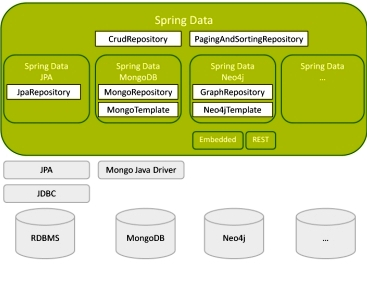
\includegraphics[width=10cm]{images/spring_data_overview}
  \caption{Architecture of Spring Data \cite{online:spring-data-overview}}
  \label{fig:spring-data-overview}
\end{figure}

\noindent JPA introduced a standard for object/relational mapping (i.e. mapping object graphs to relational database tables), with Spring Data, this support is extended to NoSQL datastores with object-like data structures.
Each type of datastore comes with its own set of annotations to provide the needed meta information for the mapping. An example of such diversity in handling different datastore mapping is reported in the code \ref{code:spring-object-mapping}.

\begin{lstlisting}[language=Java, caption=Spring Data object mapping, label=code:spring-object-mapping]
// MongoDB mapping
@Document(collection="usr")
public class User {
    @Id private String id;
    @Field("fn") private String name;
    private Date lastLogin;
    ...
}

// Neo4j mapping
@NodeEntity
public class User {
    @GraphId Long id;
    private String name;
    private Date lastLogin;
    ...
}
\end{lstlisting}

\noindent When working with data, developers generally write some DAO (Data Access Object) classes that enclose the boiler plate code for CRUD and query operations.
With JPA, CRUD operations are available through the \texttt{EntityManager} interface, queries instead needs various operations: creation, parameter set and execution.
With Spring Data, DAO classes are completely handled by the framework, requiring the user only to provide an interface of the DAO that extends a specific Spring Data repository which will map the operation to the underlying database specific implementation.
An example of this is reported in the code \ref{code:spring-dao}.

\begin{lstlisting}[language=Java, caption=Spring Data repositories, label=code:spring-dao]
public interface UserRepository extends MongoRepository<User, String> {
    List<User> findByName(String name);
    List<User> findByEmail(String email);
}
\end{lstlisting}

\subsection{PlayORM}
PlayORM \cite{online:playorm} is an open-source library developed by \textbf{Buffalo Software} with the aim of speeding up developer productivity of developing a NoSQL scalable solution. Currently supports Cassandra, MongoDB and HBase. 

\newparagraph PlayORM takes great inspiration from JPA interface but recognizes that JPA was designed fro DBMS and thus they have re-defined the JPA interface  for NoSQL purposes.
The framework thus make use of the JPA interfaces such as \texttt{EntityManager} for CRUD operations and the \texttt{Query} interface for queries but it re-define all the annotations.
Furthermore it defines an extensions of JPQL called S-JQL which stands for Scalable JQL that adds to JPQL the keyword \texttt{PARTITIONS} that allows the user to specify the specific data partition on which execute the query.

\noindent An example of entity defined with PlayORM is shown in the code snippet \ref{code:playorm-entity} and shows the similarities with the JPA approach.

\begin{lstlisting}[language=Java, caption=PlayORM object mapping, label=code:playorm-entity]
@NoSqlEntity
public class Employee {
    @NoSqlId
    private String id;
    private String lastName;
    @OneToOne
    private Phone phone;
    ...
}
\end{lstlisting}

\subsection{SOS Platform}
The SOS (Save Our Systems) Platform \cite{paper:sos-platform} is a academic project developed by Unversita' Roma Tre.

\noindent The platform achieve interoperability among NoSQL databases by defining a common interface  and a meta-layer of abstraction used to maintains entities information. Database specific handlers, read the meta-layer and translate the meta-operations to database-specific operations that are finally performed over the database instance.
The architecture is shown in figure \ref{fig:sos-architecture}.

\begin{figure}[tbh]
  \centering
  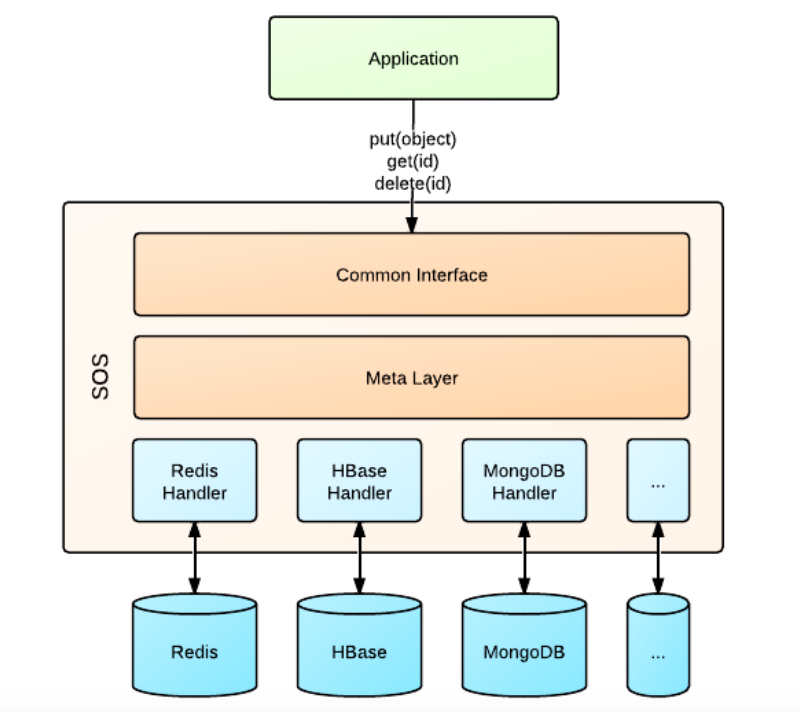
\includegraphics[width=9cm]{images/sos_architecture}
  \caption{SOS architecture \cite{paper:sos-platform}}
  \label{fig:sos-architecture}
\end{figure}

\section{The JPA interface}
\label{sec:jpa}
The Java Persistence API \cite{book:projpa2} was first released as part of Enterprise JavaBeans 3.0 in 2006. As a more general-purpose object-relational mapping facility, it was quickly recognized as such, and was expanded at the request of the community to support use in Java SE environments as well as in the other Java EE container types.

\newparagraph The Java Persistence API provides an object/relational mapping facility to Java developers for managing relational data in Java applications. Java Persistence consists of three areas:
\begin{itemize}
\item the Java Persistence API;
\item object/relational mapping meta-data;
\item the query language.
\end{itemize}

\noindent Mapping meta-data are defined by the user as Java annotations upon the classes that he wants to be mapped to the underlying database.
The user annotated classes represents entities; typically an entity represents a table in a relational database, and each entity instance corresponds to a row in that table. Entities are managed by the entity manager, the EntityManager API creates and removes persistent entity instances, finds entities by the entity’s primary key, and allows queries to be run on entities. 
The \texttt{EntityManager.createQuery} and \texttt{EntityManager.createNamedQuery} methods are used to query the datastore using Java Persistence query language queries. 

\noindent The set of all entity classes managed by the \texttt{EntityManager} instance, is defined by a \textit{peristence unit}.
Persistence units are defined in the \textit{persistence.xml} configuration file, each persistence unit is identified with a name that is unique to the persistence units scope. 

\newparagraph JPA supports two methods for expressing queries to retrieve entities and other persistent data from the database: query languages and the criteria API. The primary query language is Java Persistence Query Language (JPQL), a database-independent query language that operates on the logical entity model as opposed to the physical data model. Queries may also be expressed in SQL to take advantage of the underlying database. The criteria API provides an alternative method for constructing queries based on Java objects instead of query strings.

\noindent JPQL have its roots in the Enterprise JavaBeans Query Language (EJB QL) that was first introduced in the EJB 2.0 specification to allow developers to write portable find and select methods for container-managed entity beans. It was based on a small subset of SQL and it introduced a way to navigate across entity relationships both to select data and to filter the results.
As part of JPA was then introduced JPQL that significantly extends EJB QL, eliminating many weaknesses of its father while preserving backward compatibility.

\section{Cloud Platform Independent Model}
\label{sec:cpim}
Cloud Platform Independent Model \cite{thesis:cpim} is a Java library build in order to make Java developers able to abstract their application logic from the specific Cloud Provider on which the application will actually be deployed.

\newparagraph The aim of CPIM is to overtake the vendor lock-in that affect the current PaaS industry. Each cloud provider define its own API for the services available in the PaaS environment it expose and, even if services are the same among various providers, they expose different API. This locks an application to the PaaS environment it was developed for.

\noindent Since there is no a common interface for such services, if the need of change Cloud Provider arises, maybe due to an increased cost of maintenance, the costs of re-engineer the applciation for the new Cloud provider environment dissolves the benefit of a provider migration.

\section{Summary}
In this chapter has been introduced some of the main reasons that leads to the NoSQL database definition and why industry is so interested in those kind of technology. 
\noindent Has been presented the main projects that have born trying to define a standard NoSQL language or a standard way to communicate with different NoSQL databases, giving a quick overview of the choices made by each one. 
\noindent Finally has been presented an overview of the JPA interface specification and the CPIM library, a more general approach for a common language definition in PaaS environment.
